\documentclass{article}
\usepackage[preprint]{neurips_2024}
\usepackage[T1]{fontenc}    % use 8-bit T1 fonts
\usepackage{hyperref}       % hyperlinks
\usepackage{url}            % simple URL typesetting
\usepackage{booktabs}       % professional-quality tables
\usepackage{amsfonts}       % blackboard math symbols
\usepackage{nicefrac}       % compact symbols for 1/2, etc.
\usepackage{microtype}      % microtypography
\usepackage{xcolor}         % colors
\usepackage{graphicx}
\usepackage[section]{placeins}

\title{NLPoker: Natural Language Poker}

\author{
  Aum Kendapadi \\
  Department of Computer Science\\
  University of North Carolina at Chapel Hill\\
  Chapel Hill, NC \\
  \texttt{aum@unc.edu} \\
}

\begin{document}

\maketitle
\begin{abstract}
    We introduce \emph{NLPoker}, a framework for evaluating large language models (LLMs) as strategic agents in imperfect-information games, using natural language alone. Unlike prior poker AIs that rely on fine-tuning or reinforcement learning, \emph{NLPoker} prompts pretrained 7-8B parameter instruction-tuned LLMs—including Mistral, Llama, and Qwen models—to make poker decisions based solely on textual descriptions of the game state. We conduct extensive simulations of No-Limit Texas Hold'em without model retraining, analyzing decision-making quality across multiple temperatures. Our results show that while LLMs demonstrate surprising zero-shot competence, they exhibit significant deviations from human-like strategic behavior, including overly loose pre-flop participation, inconsistent post-flop aggression, and poor positional awareness. Nevertheless, some models, particularly Qwen2.5-7B, display resilience and effective chip stack growth in dynamic settings. \emph{NLPoker} highlights both the promise and current limitations of general-purpose language models in adversarial, high-uncertainty environments, opening avenues for future research on bridging language fluency and deep strategic reasoning.
\end{abstract}
    

\section{Introduction}

Poker is a card game blending chance, strategy, and psychology, originating in 19th-century America from earlier European and Persian games. Players wager based on hidden private cards and shared public cards, with rounds of betting driven by both probability and deception. Poker’s unique blend of imperfect information and strategic bluffing inspired early game theory work, notably by John von Neumann, and remains a canonical example of decision-making under uncertainty.

As a benchmark for AI, poker presents greater challenges than perfect-information games like chess or Go. Early computer poker programs, such as Polaris (2007), could compete with human professionals, culminating in major breakthroughs with Libratus (2017) and Pluribus (2019), which achieved superhuman performance in two-player and multiplayer No-Limit Texas Hold’em respectively. These systems combined game-theoretic strategies, reinforcement learning, and self-play to navigate the complexity of imperfect information and dynamic opponent modeling.

Meanwhile, the advent of large language models (LLMs) like GPT-4, Mistral, and Llama has revolutionized natural language understanding and generation. However, LLMs are primarily trained on text corpora, with little explicit grounding in strategic reasoning or multi-agent interaction. While they excel at producing coherent narratives, their ability to plan, bluff, and reason adversarially remains largely untested.

In this project, we introduce \emph{NLPoker}, an experimental framework where LLMs, including \texttt{mistralai/Mistral-7B-Instruct-v0.3}, \texttt{meta-llama/Meta-Llama-3.1-8B-Instruct-Turbo}, and \texttt{Qwen/Qwen2.5-7B-Instruct-Turbo}, play poker through natural language. Each model receives a textual description of the game state and responds with an action such as bet, call, or fold, expressed in natural language. This setup allows us to explore whether instruction-tuned LLMs can navigate imperfect-information strategic settings, handle adversarial interaction, and exhibit basic game-theoretic behavior, all mediated through language. \emph{NLPoker} offers an initial look at how general-purpose language models perform when linguistic fluency meets strategic reasoning.

\section{Related Work}

Recent efforts have explored large language models (LLMs) as agents for complex games like poker, moving beyond traditional game-theoretic solvers. Huang et al.\ [1] introduce PokerGPT, an end-to-end poker agent based on a lightweight LLM. PokerGPT is fine-tuned on real multi-player Texas Hold’em game transcripts (formatted as textual prompts) and further optimized via reinforcement learning from human feedback (RLHF) to refine its strategy. This approach allows the model to generate poker decisions from natural language state descriptions, achieving competitive win rates while using relatively small models. In contrast, our project \emph{NLPoker} does not involve any fine-tuning or additional training; we instead prompt pretrained LLMs directly to make poker decisions, exploring their zero-shot or few-shot strategic capabilities.

To systematically evaluate poker decision-making by LLMs, Zhuang et al.\ [2] developed PokerBench, a benchmark of 11,000 expert-designed poker scenarios. Their evaluations showed that while off-the-shelf LLMs perform poorly at optimal poker play, fine-tuning on domain-specific data substantially improves decision quality. These findings suggest that general-purpose LLMs require task-specific adaptation to reach expert-level performance. In contrast, \emph{NLPoker} investigates how far prompting alone can push pretrained LLMs toward strategic competence in imperfect-information settings without any specialized data or training.

A complementary line of research focuses on using LLMs to simulate game environments. Wu et al.\ [3] propose the Instruction-Driven Game Engine (IDGE), which trains LLMs to predict the next game state given natural language descriptions of actions and rules. In the poker domain, IDGE demonstrated that an LLM can maintain consistent game state transitions purely through text modeling. While IDGE targets accurate state evolution, \emph{NLPoker} emphasizes decision-making: given a poker situation described in language, the LLM must select an action, not just simulate the environment. Future work could combine IDGE-style state modeling with \emph{NLPoker}’s decision layer to enable fully language-driven gameplay without explicit game engines.

\section{Approach}
\begin{figure}[htbp]
\centering
\begin{minipage}{0.48\textwidth}
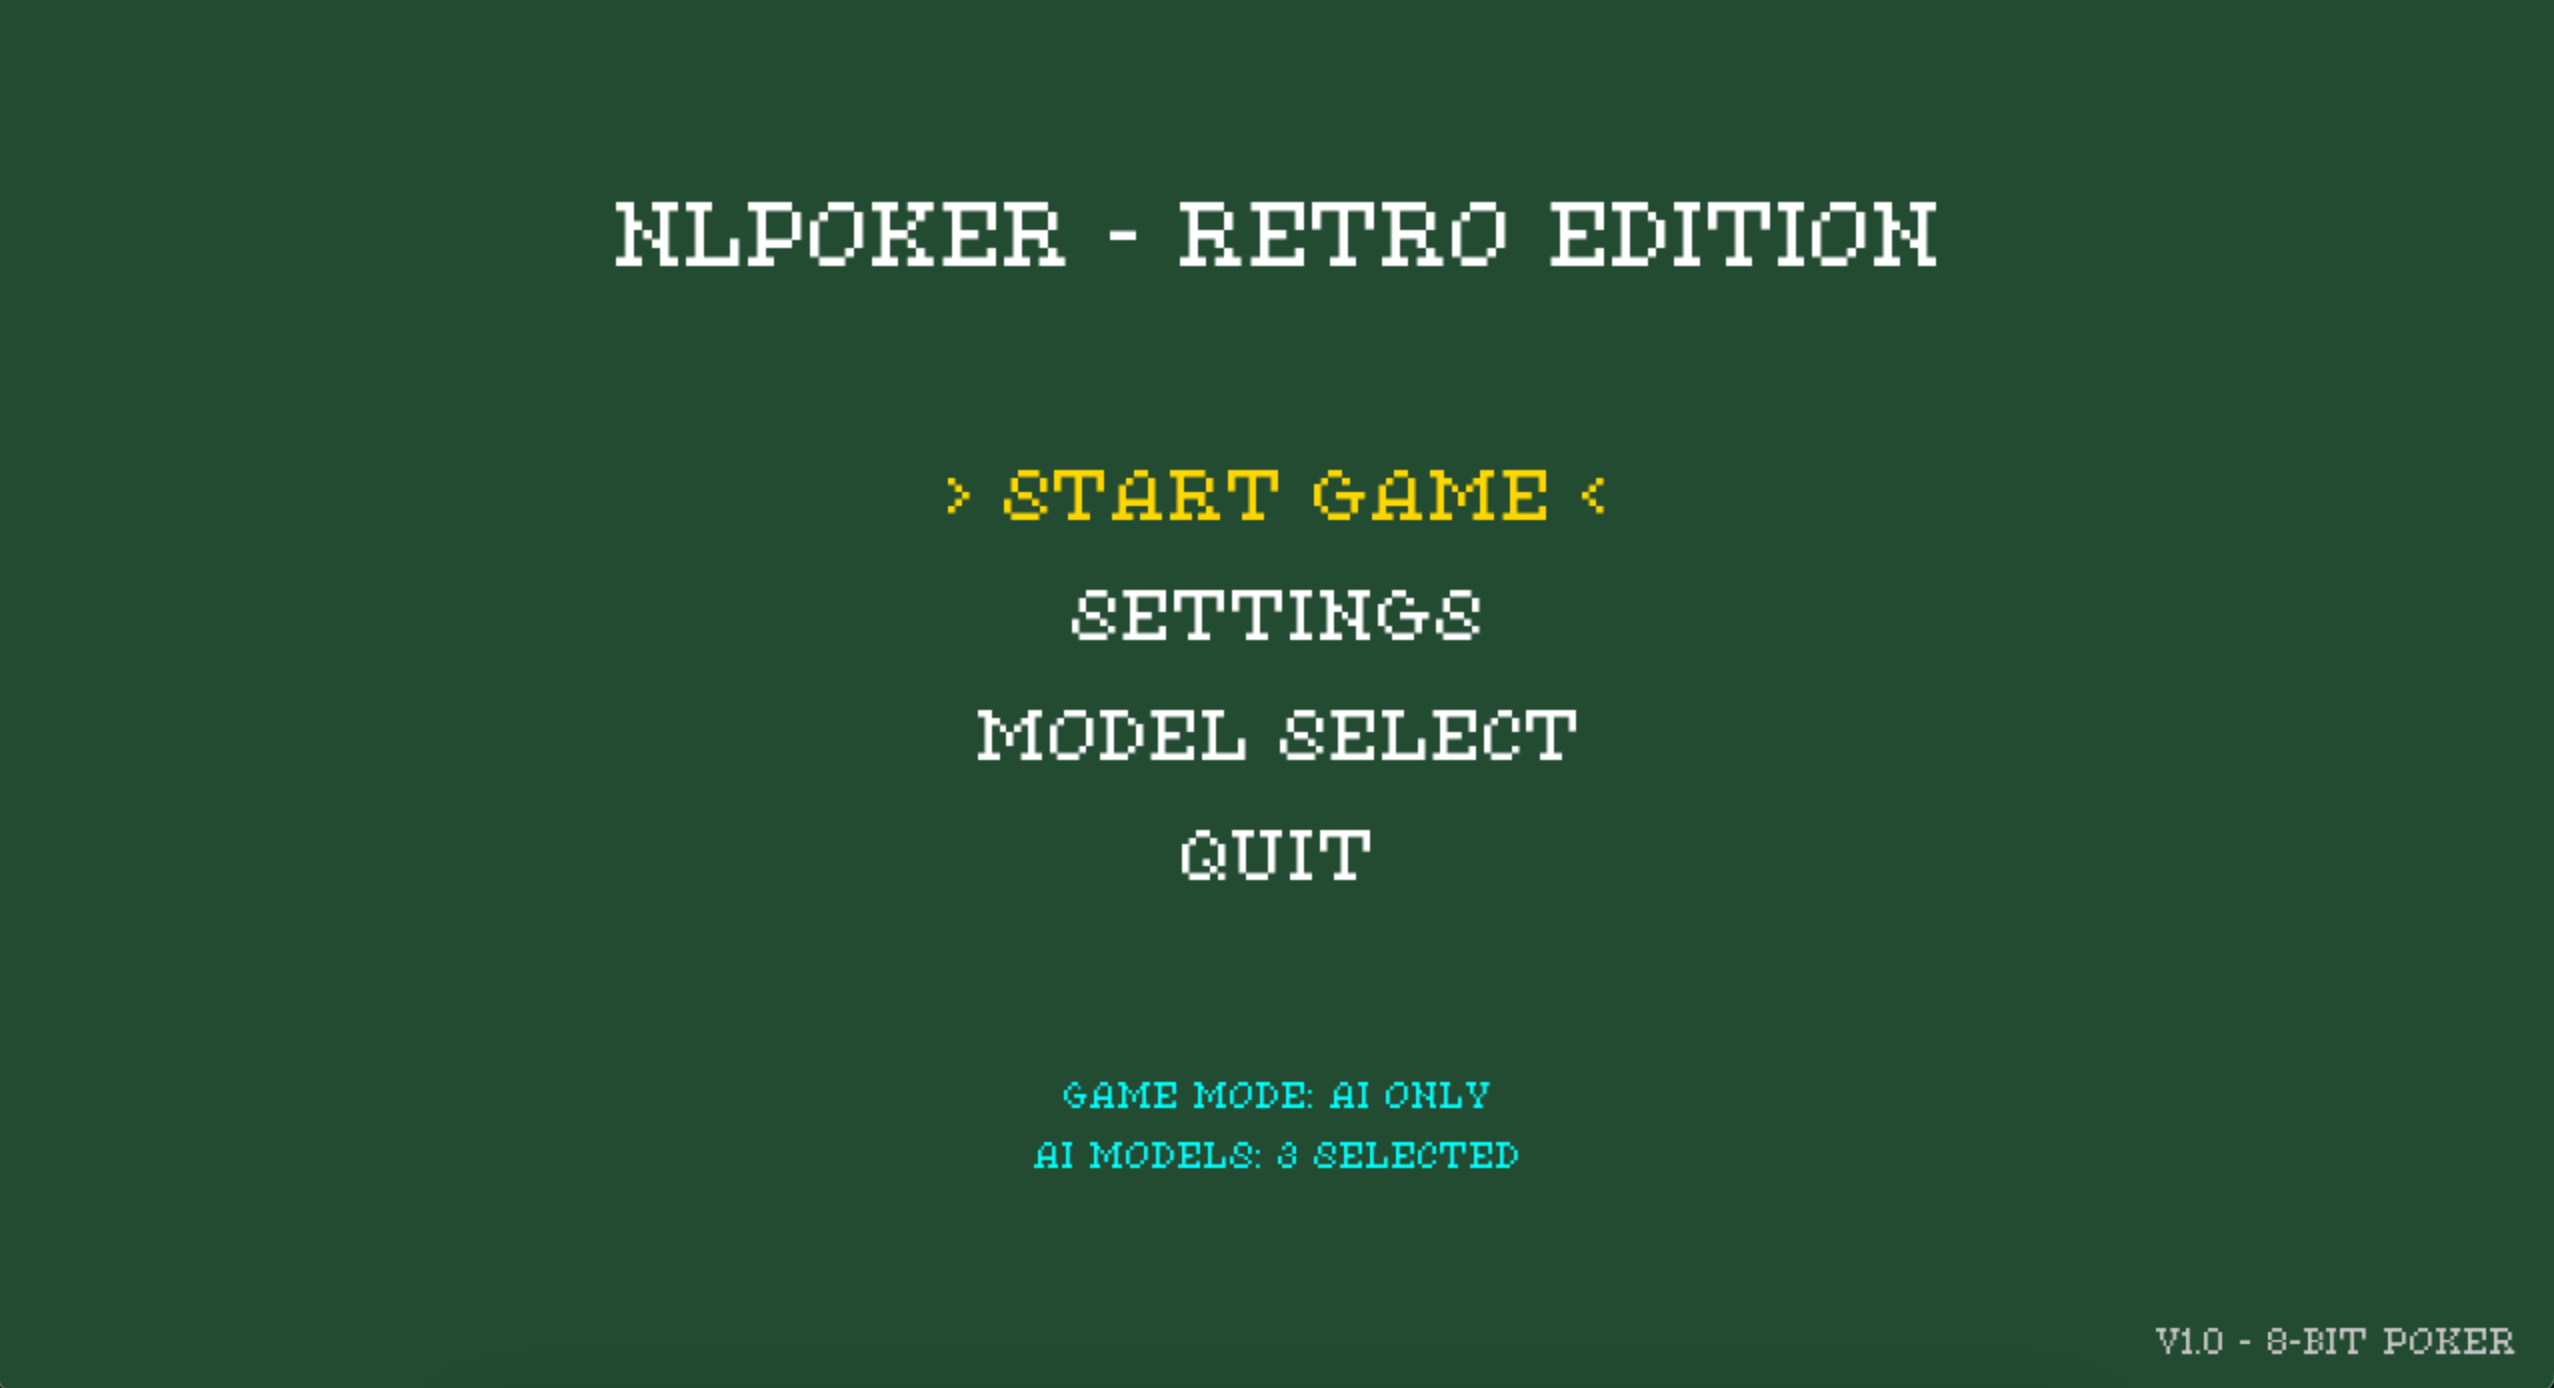
\includegraphics[width=\linewidth]{ss1.png}
\end{minipage}\hfill
\begin{minipage}{0.48\textwidth}
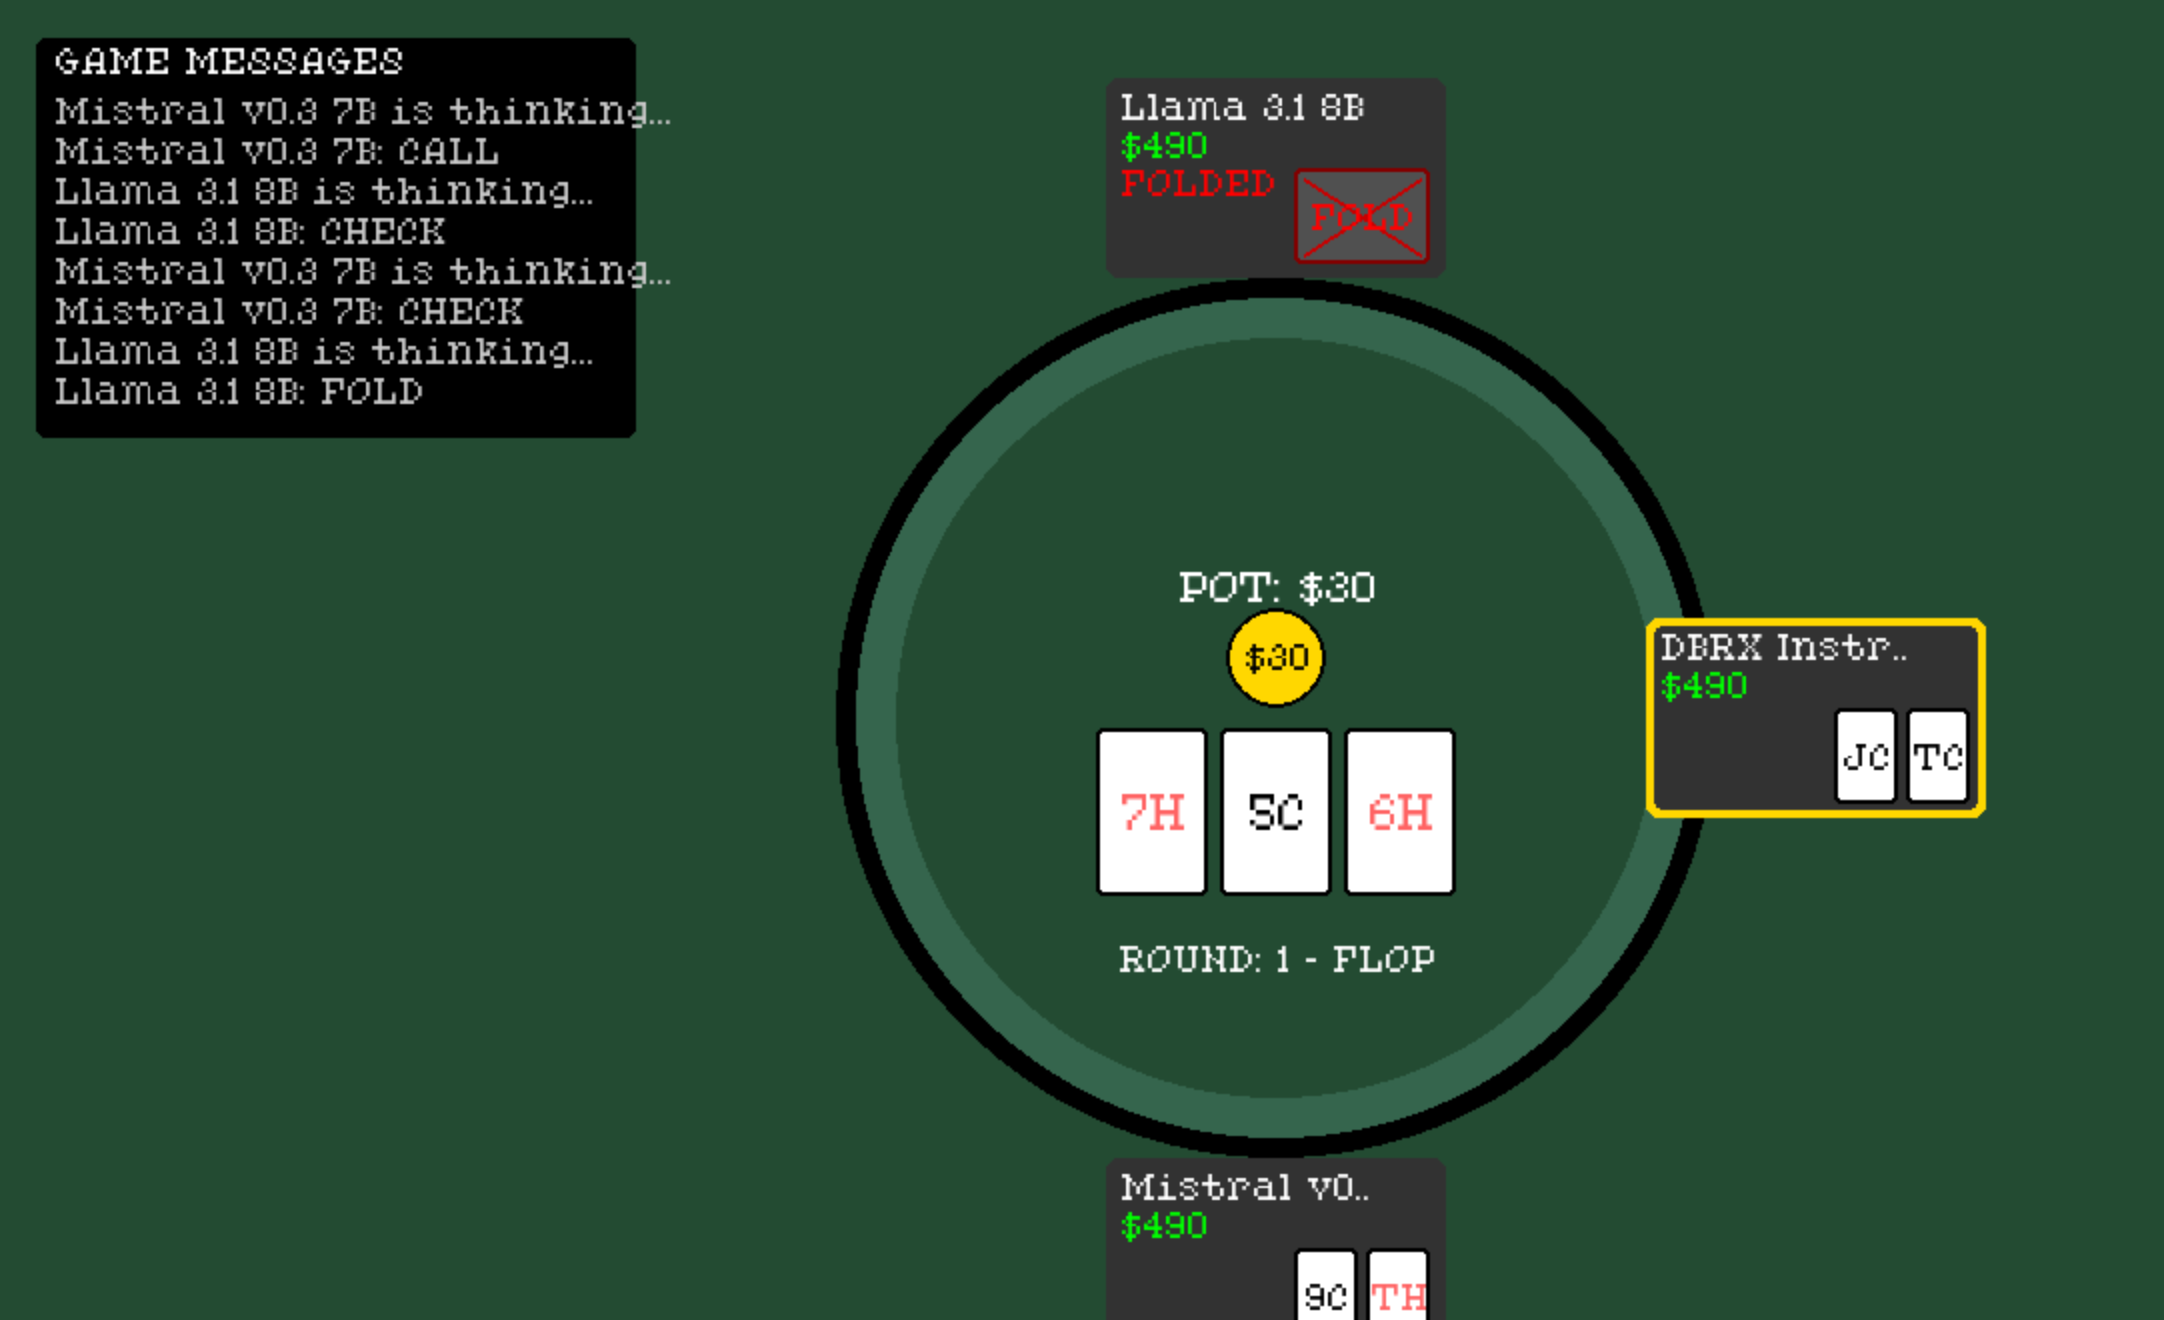
\includegraphics[width=\linewidth]{ss2.png}
\end{minipage}
\caption{Screenshots of the Pygame-based poker GUI developed using LLM-assisted coding.}
\end{figure}

The goal of this project is to explore how well large language models (LLMs) can play strategic imperfect-information games using natural language prompts alone. In contrast to prior work that fine-tunes models or trains bespoke agents through reinforcement learning, we investigate whether instruction-tuned pretrained models can make competitive poker decisions purely through prompting.

We frame Texas Hold'em poker as a language-driven task. Each game state---including board cards, pot size, player actions, and available options---is formatted into a structured natural language description and provided as input to the LLM. The model is expected to output its chosen action (e.g., ``CALL'', ``RAISE AMOUNT: 20'') without access to internal code or simulation engines. Parsing functions interpret these outputs into structured game moves.

To manage the game environment, we use the open-source \texttt{pokerlib} library for rules and flow control. Hand strength evaluation and win probability estimation are provided by the \texttt{deuces} poker library. LLM decisions are generated through API calls to Together AI, supporting a range of modern instruction-tuned models such as \texttt{meta-llama/Llama-3.3-70B-Instruct-Turbo}, \texttt{Qwen/Qwen2.5-72B-Instruct-Turbo}, and \texttt{Qwen/Qwen2.5-7B-Instruct-Turbo}.

Unlike approaches such as PokerGPT [1], which applies reinforcement learning with human feedback (RLHF), or PokerBench [2], which shows that fine-tuning improves performance, our method uses no additional training. We rely entirely on careful prompt engineering, consistent state formatting, and lightweight system instructions. This allows us to assess the \emph{zero-shot} and \emph{few-shot} strategic capabilities of general-purpose LLMs under minimal setup.

In addition to the command-line interface, we also developed a visual version of the game using \texttt{Pygame}. To accelerate development, we used the \texttt{Claude code} command-line tool to automatically generate, modify, and debug Pygame code through natural language prompts. We found that Claude was extremely effective at iterative code generation, quickly producing useful implementations and fixing its own mistakes across multiple rounds. However, this approach proved \emph{expensive}: due to the high per-token cost of Claude models and the fact that it passes large portions of the codebase as context at each step, generating and refining the Pygame GUI incurred substantial API usage fees. Nonetheless, the experiment demonstrated the growing viability of LLMs as \emph{software engineering assistants} capable of building non-trivial graphical applications through interactive prompting.

Additionally, in the command-line version of \emph{NLPoker}, we integrate a lightweight Monte Carlo simulation module using the \texttt{deuces} library to estimate each player's win probability given their private cards and the public board. After each major betting stage (preflop, flop, turn, river), the simulator samples 5,000 randomized future board completions to calculate probabilistic equities, offering insight into hand strength without full game tree exploration. This provides both players and researchers a dynamic view of evolving hand equities throughout gameplay.

\section{Execution}

To conduct our experiments, we developed a full simulation pipeline to run automated poker games between AI agents and collect detailed gameplay data. The overall software architecture, simulation parameters, and data collection mechanisms are described below.

\subsection{Software Architecture}

The \texttt{NLPoker} simulation is built around a custom subclass \texttt{SimulationTable} extending the base \texttt{Table} class from \texttt{pokerlib}. Key components include: (1) \texttt{format\_state\_for\_ai()}, converting the current game state into a structured natural language prompt for the AI model; (2) \texttt{query\_together\_ai()}, sending prompts to the Together AI API and retrieving responses; (3) \texttt{parse\_ai\_action()}, parsing the AI's textual response into structured poker actions (fold, check, call, raise); (4) \texttt{calculate\_win\_probabilities()}, running a Monte Carlo simulation (5,000 iterations) to estimate win probabilities using the \texttt{deuces} evaluator.

Each player is assigned an AI model, and the game loop proceeds as: (1) deal private hole cards, (2) format state and prompt the acting AI, (3) parse the AI's chosen action, (4) apply the action to the game engine.

Error handling is implemented at multiple levels: API request timeouts and retries; parsing validation and fallback strategies (e.g., defaulting to CHECK, CALL, or FOLD on invalid actions); and logging all errors and warnings with detailed context for debugging.

\subsection{Simulation Configuration}

We simulated \textbf{20 games} with \textbf{20 rounds} per game, using three AI models: \texttt{mistralai/Mistral-7B-Instruct-v0.3} (\textbf{Mistral v0.3 7B}), \texttt{meta-llama/Meta-Llama-3.1-8B-Instruct-Turbo} (\textbf{Llama 3.1 8B}), and \texttt{Qwen/Qwen2.5-7B-Instruct-Turbo} (\textbf{Qwen 2.5 7B}). Each player started with \$200 (buy-in), with blinds set at \$1/\$2; all games were AI-only.

Model queries used the Together AI API (90-second timeout, up to three retries). Experiments were run across three temperatures: \textbf{0.5}, \textbf{0.75}, and \textbf{1.0}, controlling the randomness of AI decision-making: (1) 0.5 for lower randomness (more deterministic behavior), (2) 0.75 for moderate randomness, (3) 1.0 for high randomness (riskier plays).

\subsection{Data Collection}

After each hand and game, structured data was recorded into CSV files under \texttt{simulation\_data/}, with each game producing a separate CSV containing hand-by-hand action logs. Recorded fields included: \texttt{hand\_id} (unique hand identifier), \texttt{street} (betting stage), \texttt{action\_number} (sequential action number), \texttt{player\_name}, \texttt{position} (early, middle, late), \texttt{action\_type} (fold, check, call, bet, raise), \texttt{action\_amount} (committed amount if applicable), \texttt{pot\_size}, \texttt{is\_all\_in} (boolean), \texttt{final\_hand} (hand classification at showdown), \texttt{won\_hand} (boolean), and \texttt{saw\_showdown} (boolean).

In addition, a comprehensive text log (\texttt{log.txt}) recorded: (1) model prompts and raw responses (if verbose mode enabled), (2) error and retry events during API communication, (3) invalid action corrections and fallback behavior, and (4) game initialization, seating, and stack events.

\subsection{Summary of Execution}

Across all temperatures, the pipeline generated: \textbf{60 games} (20 per temperature), \textbf{up to 1200 rounds} of gameplay data (subject to early eliminations), and \textbf{CSV datasets} summarizing every decision made. This setup enabled fine-grained analysis of model decision-making, strategic tendencies, risk profiles, and performance across different randomness settings.


\section{Analysis}

In this section, we present a detailed analysis of the poker simulations, examining key performance metrics across different temperatures and models. We begin with an overview of the model legend for reference, then discuss pre-flop and post-flop tendencies, bet sizing behavior, positional variation, and chip stack evolution.

\begin{figure}[!htb]
\centering
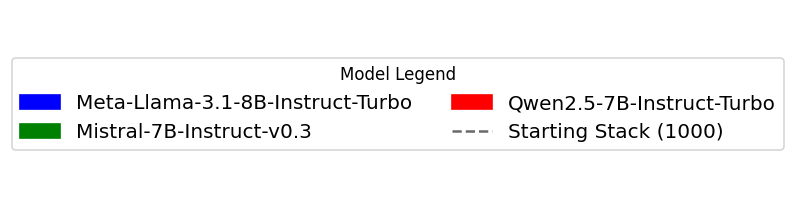
\includegraphics[width=0.7\linewidth]{plots/model_legend.png}
\end{figure}

\subsection{Pre-flop Metrics}
We measure voluntary participation and pre-flop aggression using VPIP (Voluntarily Put In Pot) and PFR (Pre Flop Raise) rates across temperatures. These metrics capture how often each model chooses to engage in or initiate betting before the flop.

\textbf{Mistral-7B} was the most aggressive (PFR > 82\%), with steady VPIP around 93--94\%. \textbf{Llama-3.1-8B} played ultra-loose (VPIP > 96\%) but passively (PFR $\sim$60\%), tightening slightly with temperature. \textbf{Qwen2.5-7B} was loose-passive, with low PFR and minor variability. Compared to human players, all LLMs were far looser pre-flop (typical human VPIP $\approx$ 20--30\%), showing minimal hand selectivity and over-participating regardless of temperature.
\begin{figure}[!htb]
    \centering
    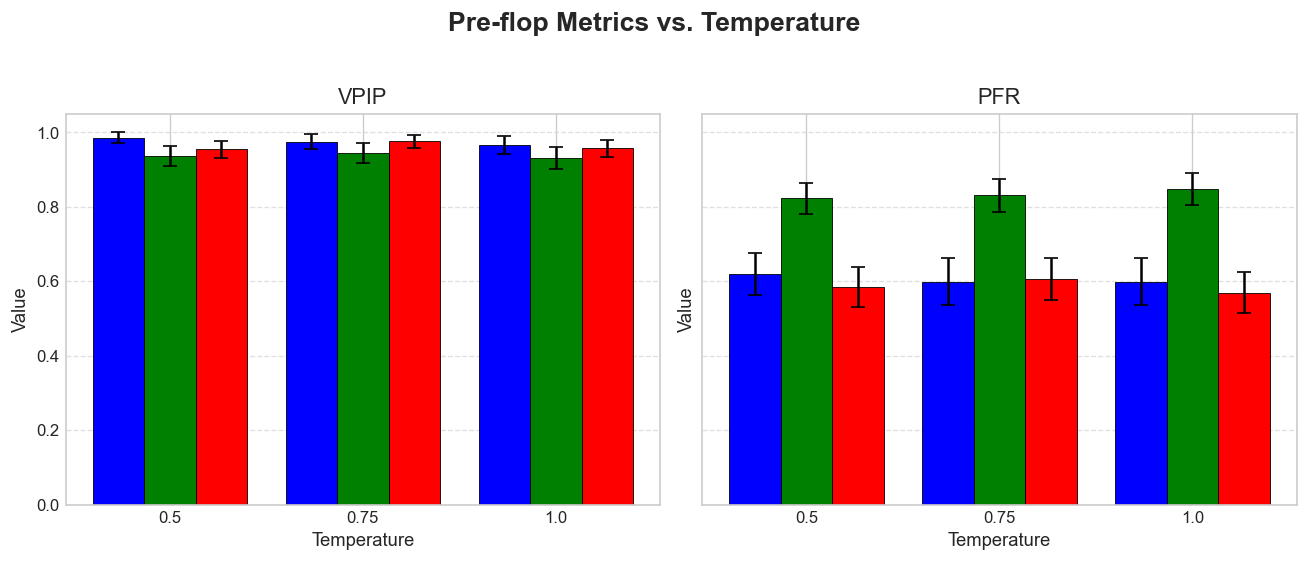
\includegraphics[width=0.8\linewidth]{plots/preflop_trends.png}
\end{figure}

\subsection{Post-flop Metrics}
We evaluate post-flop aggression frequency (AFq), Went to Showdown (WTSD) rate, and Won at Showdown (WSD) rate to understand each model's strategic choices after the flop.

\textbf{Llama-3.1-8B} showed the highest post-flop aggression (AFq $\sim$27--30\%) but had poor showdown results (WSD $\sim$16--24\%). \textbf{Mistral-7B} and \textbf{Qwen2.5-7B} were extremely passive (AFq $<$5\%) yet had better WSD rates ($\sim$23--30\%). Qwen reached the most showdowns (WTSD $>$76\%) across all temperatures. Compared to humans, LLMs were overly passive (typical human AFq $\sim$30--40\%) and showed weak post-flop pressure, leading to frequent but low-quality showdowns.
\begin{figure}[!htb]
    \centering
    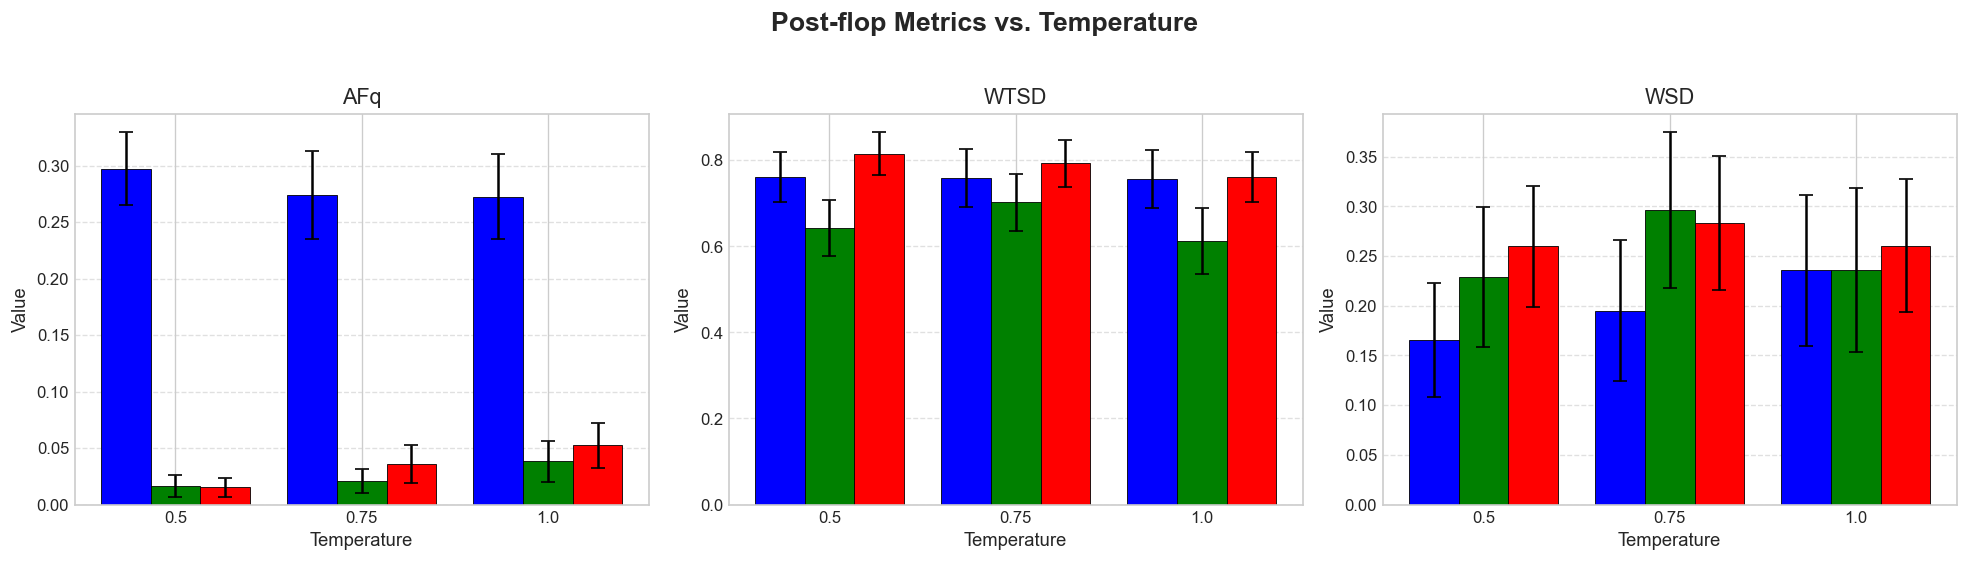
\includegraphics[width=0.8\linewidth]{plots/postflop_trends.png}
\end{figure}


\subsection{Bet Sizing Metrics}
We analyze pre-flop raise sizes (in big blinds) and post-flop bet sizing (as a percentage of the pot) to assess risk-taking and value extraction tendencies.
\textbf{Mistral-7B} made huge pre-flop raises (20--34x BB) and modest post-flop bets ($\sim$90--120\% pot). \textbf{Llama-3.1-8B} had erratic pre-flop sizing (7--11x BB) and increasingly oversized post-flop bets ($\sim$70--270\% pot at higher temperatures). \textbf{Qwen2.5-7B} bet smallest both pre- and post-flop, with consistent low sizing. Compared to humans (standard pre-flop 2--3x BB, post-flop 50--100\% pot), LLMs, especially Mistral and Llama, often overbet pre-flop and showed erratic post-flop sizing with poor pot control.
\begin{figure}[!htb]
    \centering
    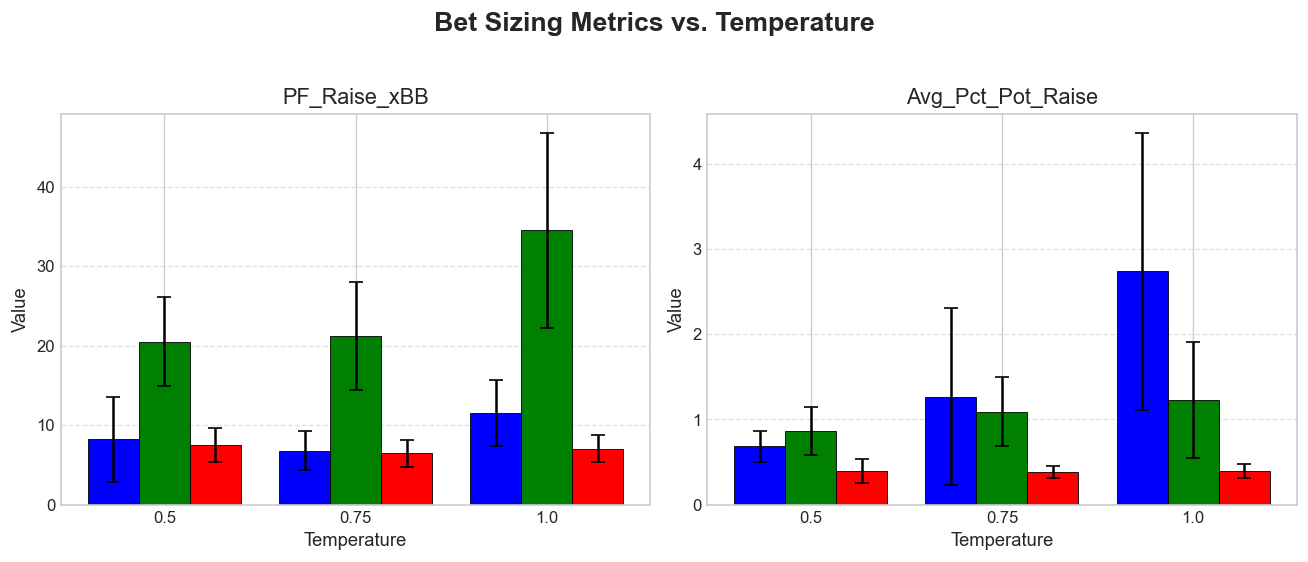
\includegraphics[width=0.8\linewidth]{plots/bet_sizing_trends.png}
\end{figure}

\subsection{Positional Metrics}
To study positional effects, we compute VPIP and PFR rates for key positions (BB, SB, BTN, BTN\_HU) across temperatures.

\textbf{Mistral-7B} showed strong positional aggression (highest PFR on BTN, SB) and adapted well across seats. \textbf{Llama-3.1-8B} was very loose everywhere but erratic in raising, especially weaker BTN\_HU play at higher temperatures. \textbf{Qwen2.5-7B} stayed loose-passive across positions, with poor PFR in heads-up (BTN\_HU). Compared to humans (tightening in early/BB, widening on BTN), LLMs ignored positional advantage, playing nearly all hands from every seat with little strategic adjustment.
\begin{figure}[!htb]
\centering
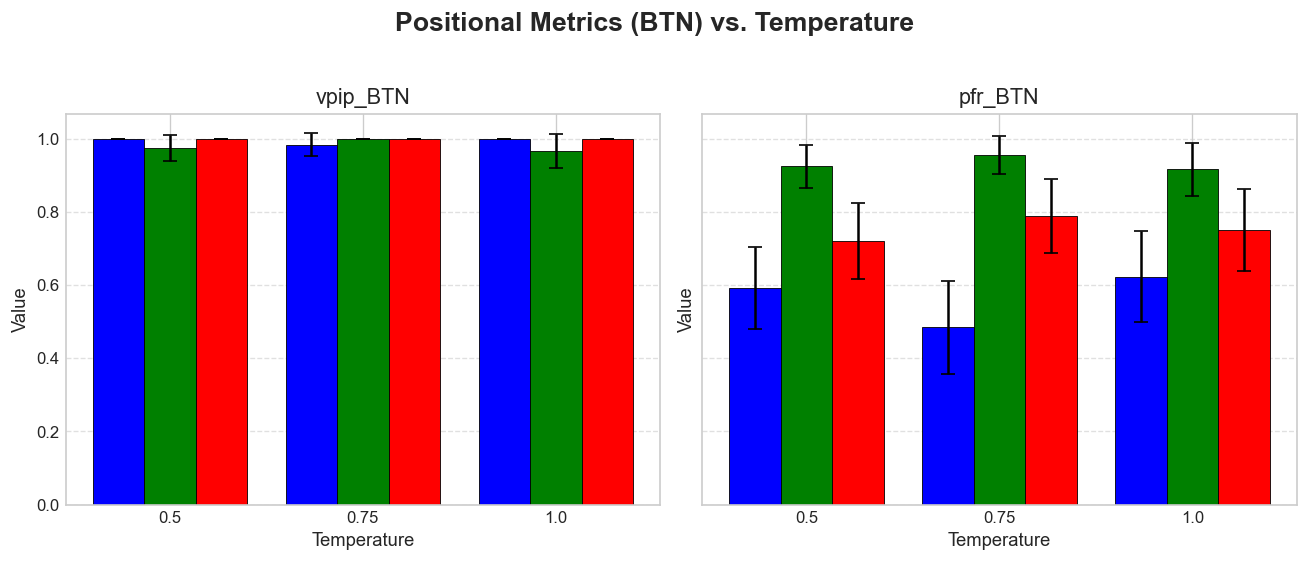
\includegraphics[width=0.48\linewidth]{plots/positional_BTN_trends.png}\hfill
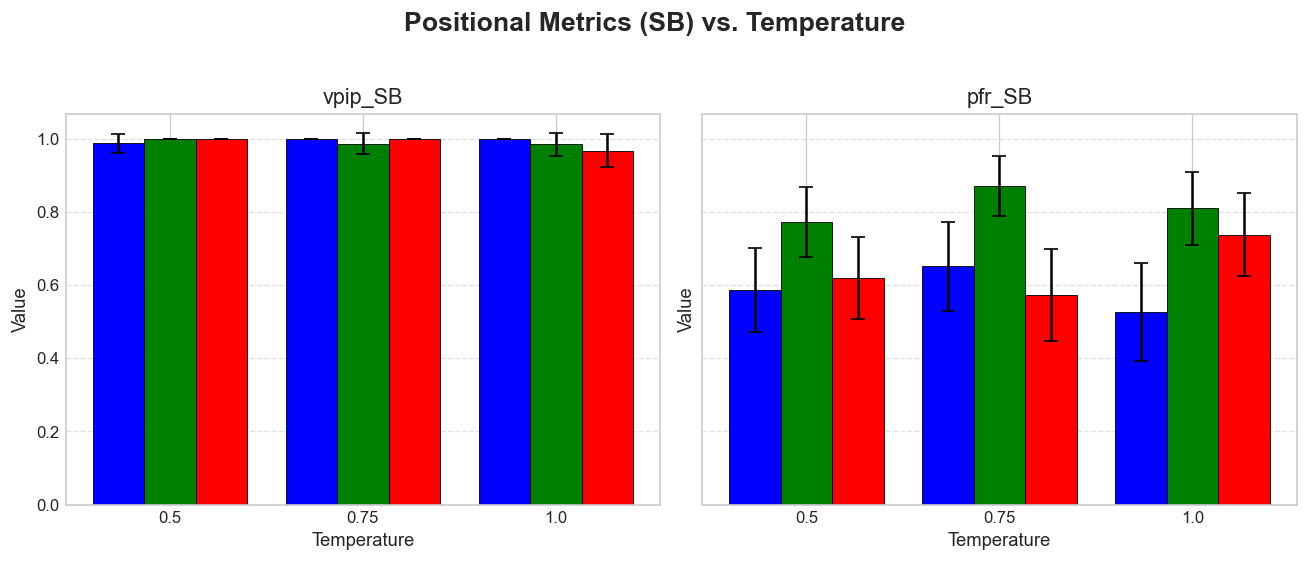
\includegraphics[width=0.48\linewidth]{plots/positional_SB_trends.png}
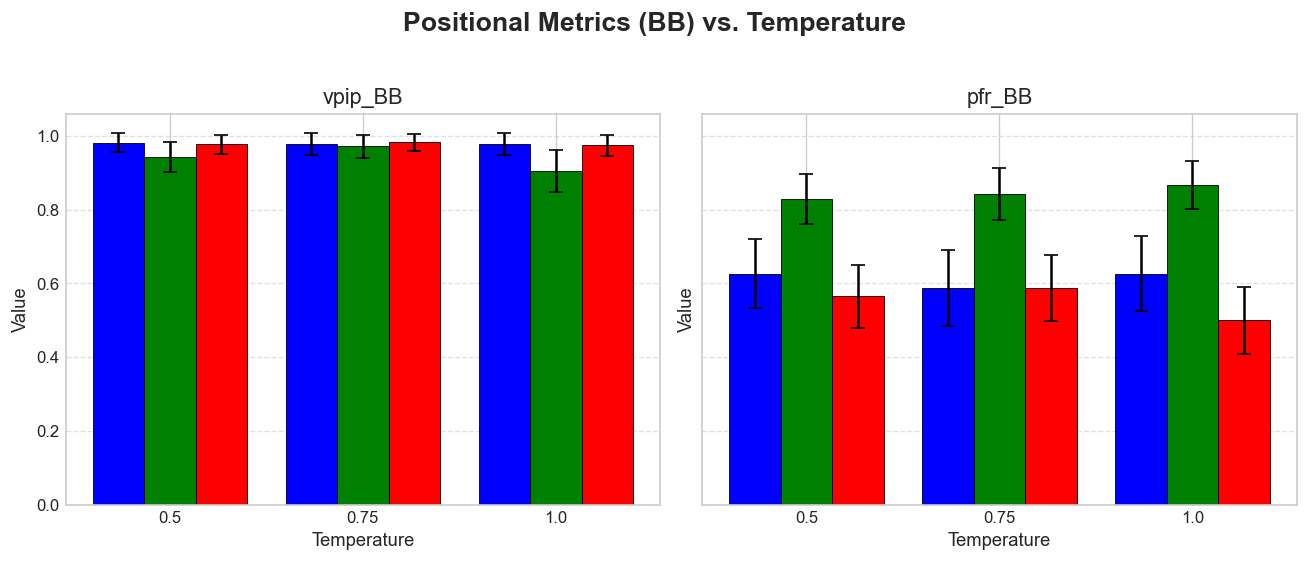
\includegraphics[width=0.48\linewidth]{plots/positional_BB_trends.png}\hfill
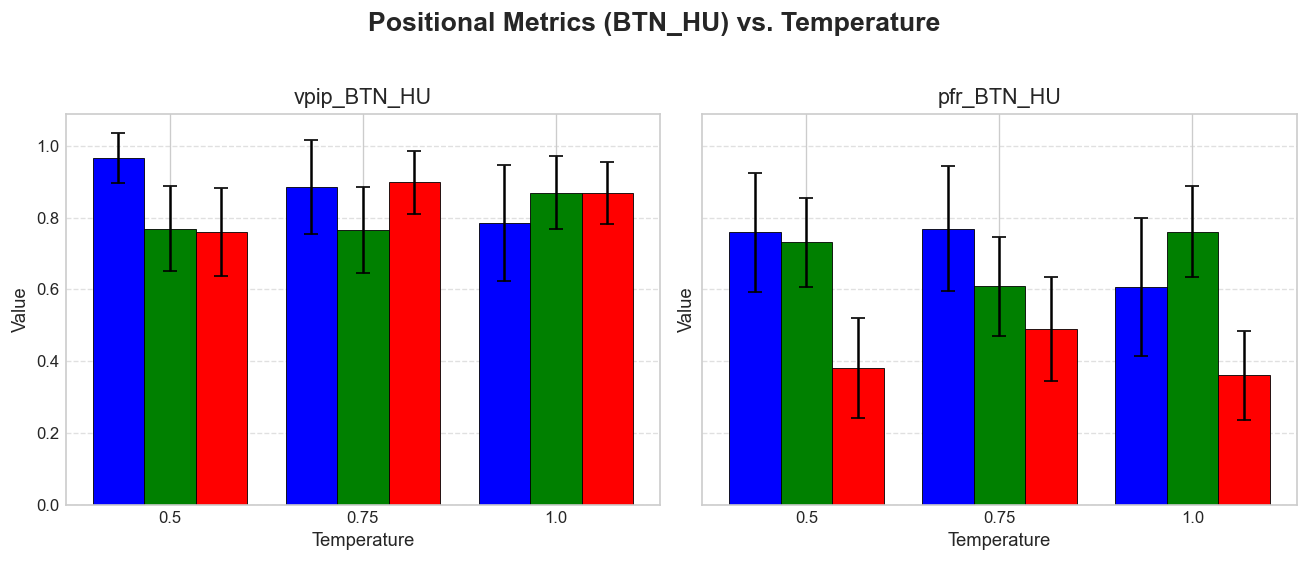
\includegraphics[width=0.48\linewidth]{plots/positional_BTN_HU_trends.png}
\end{figure}

\subsection{Chip Stack Evolution}
We examine chip stack trajectories over rounds to visualize long-term bankroll fluctuations and model resilience under different randomness settings.

\textbf{Qwen2.5-7B} (red) consistently built the largest stacks across all temperatures, showing strong survival and growth. \textbf{Mistral-7B} (green) had high volatility, with many early busts but occasional large wins. \textbf{Llama-3.1-8B} (blue) trended downward, with frequent chip loss and few strong recoveries. As temperature increased, variance grew for all models, with more wild swings and bust-outs. Compared to humans (who balance aggression with survival), LLMs showed extreme risk profiles: either doubling up or busting quickly, especially at higher randomness.
\begin{figure}[!htb]
\centering
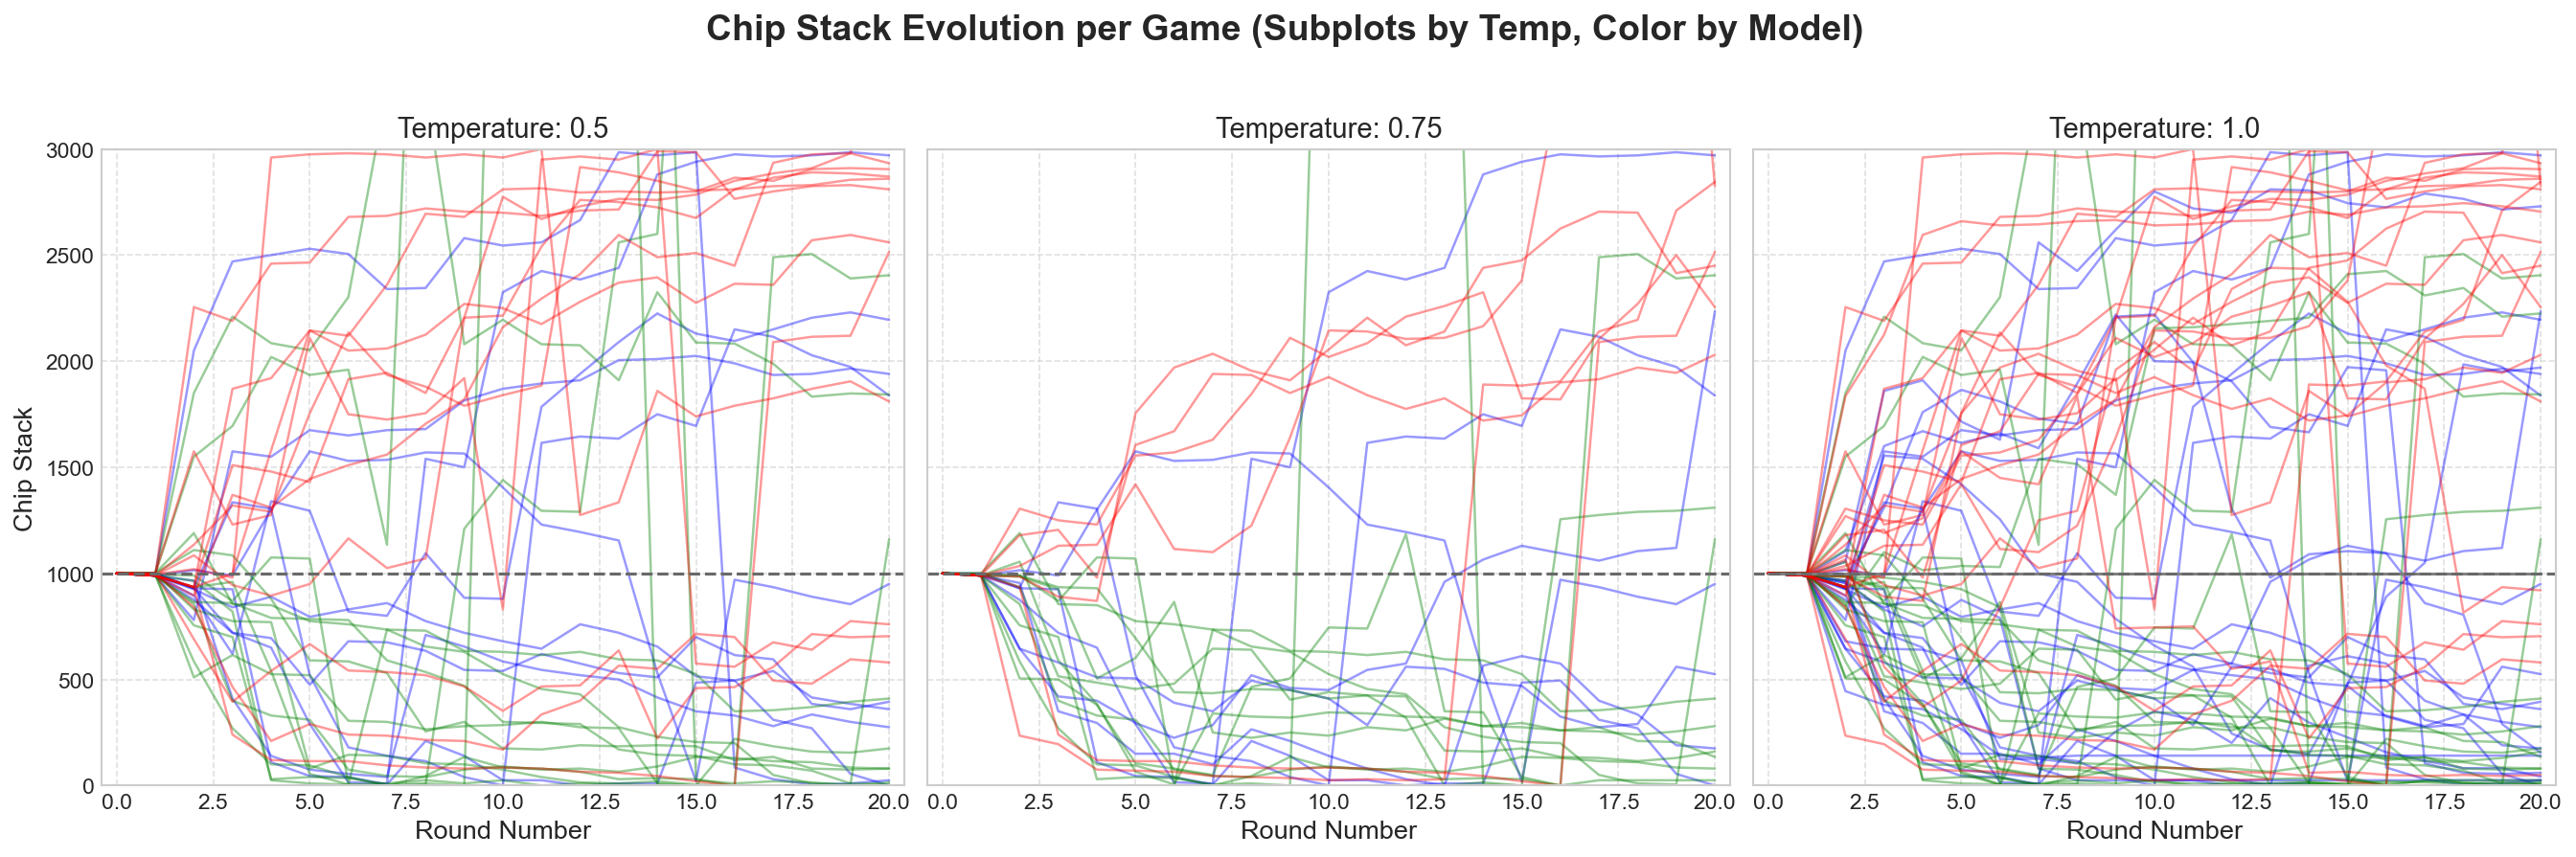
\includegraphics[width=0.9\linewidth]{plots/chip_stack_evolution.png}
\end{figure}

\section{Conclusion}

In this project, we introduced \emph{NLPoker}, a framework for studying large language models as strategic agents in imperfect-information settings through natural language interaction alone. By prompting pretrained models without any fine-tuning or reinforcement learning, we observed that instruction-tuned LLMs can meaningfully engage in poker decision-making but exhibit clear departures from human-like strategic behavior.

Across pre-flop and post-flop metrics, models like Mistral, Llama, and Qwen displayed extremely loose participation, limited aggression, and inconsistent bet sizing. While Mistral-7B showed the highest pre-flop assertiveness, Qwen2.5-7B demonstrated stronger survival instincts, often growing large chip stacks despite passive tendencies. However, all models struggled to adjust properly based on position and tended to overplay hands without selectivity.

Compared to trained human players, LLMs lacked crucial elements of disciplined strategy: hand selection, pot control, positional awareness, and post-flop aggression. Their gameplay was marked by high variance, frequent overbetting, and extreme risk profiles, especially at higher temperatures.

Overall, \emph{NLPoker} highlights both the surprising zero-shot capabilities and the clear strategic limitations of current LLMs in adversarial, imperfect-information domains. Future work could explore fine-tuning on poker-specific data, hybrid systems combining language models with search-based reasoning, or interactive multi-agent training to bridge the gap between linguistic fluency and deep strategic competence.

\paragraph{Future Work.}
While this study focused on 7B--8B scale models, future experiments should explore larger LLMs (e.g., 70B+ parameter models) to assess whether increased model capacity improves strategic depth and decision quality. Moreover, emerging \emph{thinking models} that reason through multi-step problems may offer stronger performance in imperfect-information games like poker, where deliberate planning and opponent modeling are critical. Another important direction is building formalized systems to detect, track, and analyze model errors---such as proposing illegal or incoherent moves---to better quantify reliability and intervene during gameplay when strategic failures occur. Such systems could serve as scaffolding for more robust and trustworthy LLM-based agents in competitive, rule-based environments.


\section*{References}

[1] Huang, C., Cao, Y., Wen, Y., Zhou, T.\ \& Zhang, Y.\ (2024) PokerGPT: An End-to-End Lightweight Solver for Multi-Player Texas Hold’em via Large Language Model. \textit{arXiv preprint} arXiv:2401.06781.

[2] Zhuang, R., Gupta, A., Yang, R., Rahane, A., Li, Z.\ \& Anumanchipalli, G.\ (2025) PokerBench: Training Large Language Models to Become Professional Poker Players. \textit{arXiv preprint} arXiv:2501.08328.

[3] Wu, H., Wang, Y., Liu, X., Zhao, H.\ \& Zhang, M.\ (2024) Instruction-Driven Game Engines on Large Language Models. \textit{arXiv preprint} arXiv:2404.00276.

\end{document}
